%%%%%%%%%%%%%%%%%%%%%%%%%%%%%%%%%%%%%%%%%%%%%%%%%%%%%%%%%%%%%%%%%%%%%%%%%%%
%% This file is part of the book
%%
%% Algorithmic Graph Theory
%% http://code.google.com/p/graph-theory-algorithms-book/
%%
%% Copyright (C) 2009, 2010, 2011 Minh Van Nguyen <nguyenminh2@gmail.com>
%%
%% See the file COPYING for copying conditions.
%%%%%%%%%%%%%%%%%%%%%%%%%%%%%%%%%%%%%%%%%%%%%%%%%%%%%%%%%%%%%%%%%%%%%%%%%%%

%% coloring the wheel graph W_4 using two colors
\subfigure[]{
\label{fig:vertex_coloring:wheel_graph_W_4}
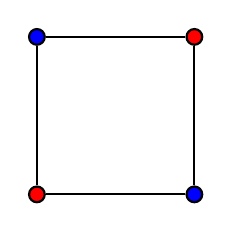
\begin{tikzpicture}
[lineDecorate/.style={-,thick},%
  nodeDecorate/.style={shape=circle,inner sep=2pt,draw,thick}]
%% nodes or vertices
\foreach \nodename/\x/\y/\fillcolor in {
  1/0/0/red, 2/2/0/blue, 3/2/2/red, 4/0/2/blue}
{
  \node (\nodename) at (\x,\y) [nodeDecorate,fill=\fillcolor] {};
}
%% edges or lines
\path
\foreach \startnode/\endnode in {
  1/2, 2/3, 3/4, 4/1}
{
  (\startnode) edge[lineDecorate] node {} (\endnode)
};
\end{tikzpicture}
}
\qquad
%%
%%
%% coloring the Petersen graph using three colors
\subfigure[]{
\label{fig:vertex_coloring:Petersen_graph}
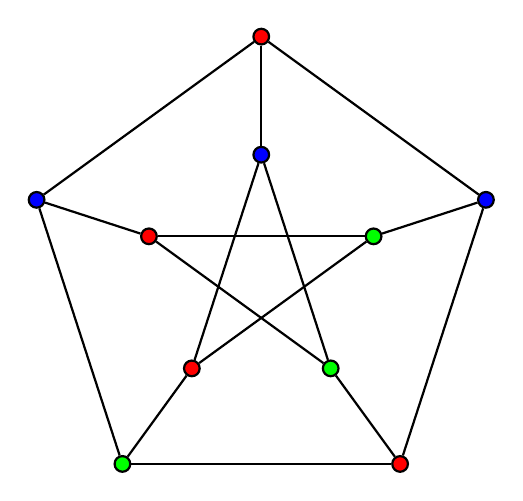
\begin{tikzpicture}
[lineDecorate/.style={-,thick},%
  nodeDecorate/.style={shape=circle,inner sep=2pt,draw,thick},%
  scale=1.5]
%% nodes or vertices
\foreach \nodename/\x/\y/\fillcolor in {
  %% inner star
  5/0.0/1.0/blue, 9/0.9510/0.3090/green, 8/0.5877/-0.8090/green,
  7/-0.5877/-0.8090/red, 6/-0.9510/0.3090/red,
  %% outer pentagon
  0/0.0/2.0/red, 4/1.9021/0.6180/blue, 3/1.1755/-1.6180/red,
  2/-1.1755/-1.6180/green, 1/-1.9021/0.6180/blue}
{
  \node (\nodename) at (\x,\y) [nodeDecorate,fill=\fillcolor] {};
}
%% edges or lines
\path
\foreach \startnode/\endnode in {
  0/1, 0/5, 1/2, 1/6, 2/3, 2/7, 3/4, 3/8, 4/0, 4/9, 5/7, 7/9, 9/6, 6/8, 8/5}
{
  (\startnode) edge[lineDecorate] node {} (\endnode)
};
\end{tikzpicture}
}
